% .:: Laden der LaTeX4EI Formelsammlungsvorlage
\documentclass[fs, footer]{latex4ei}

% Dokumentbeginn
% ======================================================================
\begin{document}

% Aufteilung in Spalten
\begin{multicols}{4}

\fstitle{Energietechnik}

% ---------------------------------------
% | 		Energietechnik	 			|
% ~~~~~~~~~~~~~~~~~~~~~~~~~~~~~~~~~~~~~~~
%=======================================================================

	\section{Physikalische Grundlagen}
	$P = F \cdot v = M \cdot \omega$ \\
	$\omega := \frac{\diff \phi}{\diff t} = 2 \pi n = 2 \pi f = \frac{v}{r}$ \\


	\section{Lastganglinien}
	$T_n$: Nennbetriebsdauer\\
	$T_a$ Ausnutzungsadauer\\
	$T_{ben}$: Benutzungsdauer\\
	$P_{max}$: Höchstalast\\
	$W = \int_0^{T_n} P(t) \diff t = P_{mittel} T_n = P_n T_a = P_{max} T_{ben}$\\
	
	\section{Wechel-/Drehstromsystem}


		\subsection{Wechselstromsystem}
		Phasenwinkel $\varphi = \varphi_u - \varphi_i$ \qquad Kreisfrequenz: $\omega = 2\pi f$\\
		
		
		Physikalische Zeitsignale:\\
		$u(t) = \hat u \cos(\omega t + \varphi_u) = U \sqrt{2} \cos(\omega t + \varphi_u)$\\
		$i(t) = \hat i \cos(\omega t + \varphi_i) = I \sqrt{2} \cos(\omega t + \varphi_i)$\\
		\\
		Komplexes Zeitsignal(Drehzeiger): $\vec u(t) = \hat u \exp\big(\i (\omega t + \varphi_u)\big)$, 
		$u(t) = \Re(\vec u(t))$\\
		
	
		Scheitelwert $\hat u$, Effektivwert $U = \sqrt{\frac{1}{T} \int_{t_0}^{t_0 + T} u^2(\tau) \diff \tau}$,
		bei Sinus $U = \frac{\hat u}{\sqrt{2}}$\\
		Effektiver Zeiger: $\vec U = U \exp(\i \varphi_u)$\\
		
		$\vec U \cdot \sqrt{2} \exp(\i \omega t) = \vec u(t)$	
	

	
		\subsection{Komplexe Leistung}
		$P = \frac1T \int_0^{T} p(t) \diff t = \frac1T \int_0^{T} u(t) \cdot i(t) \diff t$\\
		\begin{tabular}{lll}
		Wirkleistung & $P = \Re(\vec S) = U I \cdot \cos(\varphi)$ & [W] \\
		Blindleistung & $Q = \Im(\vec S) = U I \cdot \sin(\varphi)$ & [Var]\\
		Scheinleistung & $S = U \cdot I = \sqrt{P^2 + Q^2}$ & [VA]\\
		\end{tabular}
		\pbox{8.0cm}{
		Scheinleistung: $\vec S = \vec U \cdot \vec I^*$ \\ $\norm{\vec S} = S = \sqrt{P^2 + Q^2}$\\ Leistungsfaktor $\lambda = \frac{|P|}{S} = \cos(\varphi)$ } \qquad
		\pbox{4cm}{ \includegraphics{./img/leistung.pdf} }\\
		
		Scheinleistung schwingt mit doppelter Netzfrequenz!
		$p(t) = P + S \cdot \cos(2\omega t + \varphi_u + \varphi_i)$\\
		$\tilde {\vec S} = \vec U \cdot \vec I$\\

		\begin{tabular}{ll}
		Impedanz(Scheinwiderstand) & Admittanz(Scheinleitwert)\\
		$\vec Z = R + \i X = \exp(\i \varphi_Z)$ & $\vec Y = G + \i B = \exp(\i \varphi_Y)$\\
		$\underset{\text{Impedanz}}{Z(j\omega)} = \underset{\text{Resistanz}}{R(j\omega)} + \underset{\text{Reaktanz}}{jX(j\omega)}$ & 	$\underset{\text{Admittanz}}{Y(j\omega)} = \underset{\text{Konduktanz}}{G(j\omega)} + \underset{\text{Suszeptanz}}{jB(j\omega)}$\\
		$\vec U = \vec Z \cdot I $ & $\vec I = \vec Y \cdot \vec U$\\

		\end{tabular}



		\subsection{Drehstromsystem}
		Drehoperator: $\vec a = \exp\bigl(\i \frac{2}{3} \pi \bigr)$ \qquad $\vec a^0 = \vec a^3 = 1$ \quad $\vec a^* = \vec a^2$\\
		
		% Zeigerdiagramm mit Drehoperatoren
		
		Effektive Leiter-Erdspannungen: $\vec U_1,\vec U_2,\vec U_3$\\
		Effektive Außenleiterspannungen: $\vec U_{12},\vec U_{23},\vec U_{31}$\\
		symmetrischer Betrieb:\\
		$U = |U_1| = |U_2| = |U_3|$\\
		Netznennspannung: $U_n = |U_{12}| = |U_{23}| = |U_{32}| = \sqrt{3} U$\\
		Gesamte Leistung: $\vec S = \sqrt{3} \cdot \vec U_n \cdot \vec I^\star$\\
		bei symmetrischem Betrieb: $\vec S = 3 \cdot \vec U \cdot \vec I$\\
		bei unsymmetrischem Betrieb: 
		\[\vec S = \vec U_1 \cdot \vec I_1^\star + \vec U_2 \cdot \vec I_2^\star + \vec U_3 \cdot \vec I_3^\star\]
		
		Komplexe Wechselleistung:
		\[\tilde{\vec S} = \vec U_1 \cdot \vec I_1 + \vec U_2 \cdot \vec I_2 + \vec U_3 \cdot \vec I_3\]
		Tatsächlicher Leistungsfluss:
		\[p(t) = \operatorname{Re} \left\{ \vec S \right\} + \operatorname{Re} \left\{\tilde{\vec S} e^{j 2 \omega t} \right\}\]


	\section{Elektrische Maschinen}
	können als Motoren oder Generatoren benutzt werden. ($\eta > 90\%$)\\
	Besteht aus Stator(Ständer),Rotor(Läufer), Anker und Welle.\\
	$n:$ Drehzahl; $M:$ magn. Moment\\


		\subsection{Der Transformator}
		
		\includegraphics[scale=.2]{./img/ersatzschaltbild_transformator.pdf} \\

		\begin{tabular}{cl}
		ü & Übersetzung \\
		$"u_r$ & Bemessungsübersetzung \\
		$U_{r1T}$, $U_{r2T}$ & Bemessungsspannungen \\
		$S_{rT}$ & Bemessungsleistung \\
		$U_{K}$ & Kurzschlussspannung \\
		$u_k$ & bezogene Kurzschlussspannung \\
		$u_r$ & bezogener Wirkspannungsabfall \\
		$P_{Cu}$ & Kupferverluste \\
		$P_{Fe}$ & Eisenverluste \\
		$Z_k$ & Kurzschlussimpedanz
		\end{tabular}

		Zur Berechnung wird oft $"u_r$ anstelle von $"u$ eingesetzt, da ersteres meist unbekannt ist. Die Bemessungsübersetzung findet sich aber auf dem Typenschild. \\
		$\vec U^b = "u \vec U$ \\
		$\vec I^b = \frac{1}{"u} \vec I$ \\
		$\vec Z^b = "u^2 \vec Z$ \\
		$"u = \frac{W_1}{W_2}$ \\
		$"u_r = \frac{U_{r1T}}{U_{r2T}}$ \\
		$u_k = \frac{U_{K}}{U_{r1T}}$ \\
		$Z_k = \frac{U_{kT}}{\sqrt{3}\cdot I_r} = u_k \frac{U_{r1T}^2}{S_{rT}}$ \\
		$u_r = \frac{U_{rT}}{U_{r1T}}$ \\
		$R_k = P_{Cu} \left( \frac{U_{r1T}}{S_{rT}} \right)^2$ \\
		$R_k = u_r \frac{U_{r1T}^2}{S_{rT}}$ \\
		$Z_k = \sqrt{R_k^2 + X_k^2}$ \\
		$R_{Fe} = \frac{U_{r1T}^2}{P_{Fe}}$ \\
		$I_{W0} = \frac{P_{Fe}}{\sqrt{3} U_{r1T}}$ \\
		$I_h = \sqrt{I_{10}^2 - I_{W0}^2}$ \\
		$X_h = \frac{U_{r1T}}{\sqrt{3} I_h}$
	
	
		\includegraphics{./img/LeitungTrafo.pdf}
	
		\subsection{Gleichstrommaschine}
		
		\begin{tabular}{cl}
		$p$ & Polpaarzahl \\
		$z$ & Anzahl der Schaltstufen \\
		$\lambda$ & Schaltverhältnis \\
		$U$ & Ankerklemmenspannung \\
		$U_i$ & Im Anker induzierte Spannung \\
		$K_1$, $K_2$ & Maschinenkonstanten \\
		$\Phi$ & magnetischer Fluss durch den Anker \\
		$I_A$ & Ankerstrom \\
		$R_A$ & Widerstand der Ankerwicklungen \\
		$I_E$ & Erregerstrom
		\end{tabular}
		
		\subsubsection{Grundgleichungen}
		$U_A = U_i + (R_A + R_v) I_A = U_i + RI$\\
		$U_i = K_1 \Phi n$\\
		$M = K_2 \Phi I_A$\\
		$\Phi = f(I_E)$\\
		falls verlustfrei: $K_1 = 2 \pi K_2$ \\
		falls im linearen Bereich: $\Phi = K_3 I_E$ \\
		
		\begin{center}
		\includegraphics[scale=.2]{./img/ersatzschaltbild_gleichstrommaschine.pdf}
		\end{center}
		
		\subsubsection{Anlaufen mit Vorwiderständen}
		$R_{A_,z-1} = R_A + R_{V1}$, $R_{A_,z-1} = R_A + R_{V1} + R_{V2}$, ..., $R_{A,0} = R_A + R_{V1} + \hdots + R_{Vz}$ \\
		$\lambda = \frac{M_{max}}{M_{min}} = \frac{R_{A,Z-1}}{R_{A,Z}}$ \\
		$ z = \log_\lambda \frac{R_{A0}}{R_A}$
		
		% Bild der Vorwiderstände
		
		\subsubsection{Fremderregt}
		$n = \frac{U}{ K_1 \cdot \Phi} - \frac{R}{K_1 \cdot K_2 \cdot \phi^2}M$\\

		mit Abkürzungen: \\
		$n_0 = \frac{U}{K_1 \Phi}$ \\
		$M_A = \frac{U K_2 \Phi}{R}$ \\
		$n = n_0 - n_0 \frac{M}{M_A}$
		
		% Ersatzschaltbild
		
		\subsubsection{Reihenschluss}
		$M = \frac{K_2}{K_3} \Phi^2$ \\
		$n = \frac{U}{\sqrt{2 \pi K_1 K_3}} \frac{1}{\sqrt{M}} - \frac{R}{K_1 K_3}$
		
		% Ersatzschaltbild
		
		\subsection{Synchronmaschine}
		
		\begin{center}
		\includegraphics[scale=.2]{./img/ersatzschaltbild_synchronmaschine.pdf}
		\end{center}
		
		Synchrone Reaktanz $X_d = \omega \cdot (L_h + L_\sigma)$\\
		$X_d \cdot I_w = U_p \sin(\vartheta_M)$\\
		$X_d = x_d \frac{U_r^2}{S_r}$ \\
		\begin{tabular}{ll}
			Übereregung & Untereregung\\ \midrule
			SMA wirkt wie Kapazität & SMA wirkt wie Induktivität\\
			gibt induktive Blindleistung ab & nimmt induktive Blindleistung auf\\
		\end{tabular}
		
		Kippmoment $M_k$; Betrieb bei ca. $\frac{2}{3} M_k \Rightarrow \vartheta_M < 42^\circ$\\
		
		\begin{center}
		\includegraphics[scale=.6]{./img/synchronmaschine_betriebsbereiche.jpg}
		\end{center}
		
		\subsection{Asynchronmaschine}
		
		\begin{center}
		\includegraphics[scale=.2]{./img/ersatzschaltbild_asynchronmaschine.pdf}
		\end{center}
		 
		 $s = \frac{n_0 - n}{n_0}$ \\
		 $M = \frac{3}{2 \pi n_0} \frac{I^2 R_l}{s}$ \\
		 $n_0 = \frac{f}{p}$ \\
		 $M = \frac{2 M_k}{\frac{s}{s_k} + \frac{s_k}{s}}$


		Anlauf nur möglich falls $M_A < M_{an}$\\
		$U$ kann nicht beliebig erhöht werden $\Ra$ Fluss wird kleiner $\Ra$ Moment wird kleiner.\\
		
		$\eta = 1 - s$ \\
		$s_k = \frac{R_L}{X_\sigma}$ \\
		$M_k = \frac{3}{2 \pi n_0} \frac{U^2}{2 X_\sigma}$
		
		
	\section{Elektrische Energieübertragung}
	
		\subsection{Leitungsmatrizen}
		
		% einphasiges ESB für den symmetrischen Betrieb
		
		\[\begin{pmatrix} \vec U_1 \\ \vec U_2 \\ \vec U_3 \end{pmatrix} = \begin{pmatrix} \vec Z_d & \vec Z_k & \vec Z_k \\ \vec Z_k & \vec Z_d & \vec Z_k \\ \vec Z_k & \vec Z_k & \vec Z_d \end{pmatrix} \begin{pmatrix} \vec I_1 \\ \vec I_2 \\ \vec I_3 \end{pmatrix}\]
		Im symmetrischen Betrieb kann im einphasigen ESB $Z_b$ als Leitungsimpedanz eingesetzt werden: $\vec Z_b = \vec Z_d - \vec Z_k$
		
		\subsection{Leitungsbetrachtungen}

		Leitungswinkel: $\vartheta = \varphi_{u1} - \varphi_{u2}$


		\subsection{Vereinfachte Leitungsbetrachtung}
		
		% einphasiges ESB
		
		Vernachlässigung von Queradmittanzen $\Ra$ $I_{in} = I_{out}$\\
		Längsspannungsabfall: $\Delta U = \begin{cases} R \cdot I_w + \omega L_b I_b & \text{ohmsch induktive Last} \\ R \cdot I_w - \omega L_b I_b  & \text{ohmsch kapazitive Last} \end{cases} $\\
		Querspannungsabfall: $\delta U = \begin{cases} \omega L_b I_w - R I_b & \text{ohmsch induktive Last} \\ \omega L_b I_w + R I_b & \text{ohmsch kapazitive Last} \end{cases}$\\
		$P_V = P_1 - P_2 = 3 I^2 R$ \\
		$Q_V = Q_1 - Q_2 = 3 I^2 \omega L_b$ \\
		$\vec U_1 = \vec U_2 + \Delta U + j \delta U$ \\
		falls $R << \omega L_b$ \quad $\Ra \vec U_{12} = j \omega L_b (I_w + j I_b)$
		
		\subsection{Verlustfreie Hochspannungsfernleitung}
		
		% einphasiges ESB
		
		$Z_W = \sqrt{\frac{\omega L'_b}{\omega C'_b}}$ \\
		$\beta = \sqrt{\omega L'_b \omega C'_b}$ \\
		$\vec U_1 = \vec U_2 \cos (\beta l) + j Z_W \sin (\beta l) \vec I_2$ \\
		$\vec I_1 = j \frac{\vec U_2}{Z_W} \sin (\beta l) + \vec I_2 \cos (\beta l)$ \\
		$P_{nat} = \frac{U_n^2}{Z_W}$ \\
		
		\begin{tabular}{lcc}
		 & elektrisch kurz \\
		Freileitung & $\le 200$ km \\
		Kabel & $\le 100$ km
		\end{tabular}

		
		\begin{tabular}{lll}
		& $\vec Z_l$ & $\frac{\vec Y_q}{2}$\\[0.5em] \midrule
		el. lange Leitung & $\i Z_w \sin(\beta l)$ & $\frac{\cos(\beta l) -1}{\i Z_w \sin(\beta l)}$\\[0.5em]
		el. kurze Leitung & $\i \omega L'_b I$ & $\frac{\i \omega C'_b l}{2}$\\[0.5em]
		\end{tabular}
		
		Bei Übertragung der natürlichen Leistung: \\
		$\vec U_1 = \vec U_2 e^{j \beta l}$ \\
		$\vec I_1 = \vec I_2 e^{j \beta l}$ \\


	\section{Hochspannungstechnik}
		\subsection{Gasdurchschlag}
		$p = \frac{r + d}{r}$ \\
		$r$: Radius des stärker gekrümmten Betriebsmittels \\
		$\eta = \frac{E_{mittel}}{E_{max}} = \frac{U/s}{E_{max}}$ \\
		$U_i = E_{dh} \cdot s \cdot \eta$ \\
		$U_s = E_s \cdot s$ \\
		$U_d = \max\{U_i, U_s\}$ \\
		$E_{dh,Luft} = 25 \hdots 50 \frac{kV}{cm}$ \\
		\begin{tabular}{l|c}
		 & $E_s / \frac{kV}{cm}$ \\ \hline
		 positive Gleichspannung & $4,5$ \\ \hline
		 negative Gleichspannung & $5 \hdots 10$ \\ \hline
		 Wechselspannung & $4,5$
		\end{tabular}

	\subsection{Lichtbogen}
	\includegraphics{./img/Lichtbogen.pdf}\\
	Ayrton-Gleichung: $U_B = U_0 - R \cdot I_B = a + bl + \frac{c+dl}{I_B}$\\
	Determinante = 0 \quad $\Longrightarrow$ \quad $R \ra \text{max};\ U_{B} \ra \text{min}$\\
	\\
	Löschblechabstand von wenigen mm: $U_B = 20$V:\\
	$n \cdot U_B > U_0$






% Ende der Spalten
\end{multicols}

% Dokumentende
% ======================================================================
\end{document}
